\section{Fairness in machine learning}

\begin{frame}
  \frametitle{Bail decisions}
  \centering
  \begin{columns}
    \begin{column}{0.5\textwidth}
      \centering
      \begin{tikzpicture}
        \node at (0,0) (judge) {\includegraphics[width=0.3\columnwidth]{../figures/judge}};
        \uncover<2->{
          \node at (-2,-2) (jail) {\includegraphics[width=0.3\columnwidth]{../figures/jail}};
          \draw[->] (judge) -- (jail);
        }
        \uncover<3->{
          \node at (2,-2) (bail) {\includegraphics[width=0.3\columnwidth]{../figures/bail}};
          \draw[->] (judge) -- (bail);
        }

        \uncover<4->{
          \node at (-2,-4) (trial) {\includegraphics[width=0.3\columnwidth]{../figures/trial}};
          \draw[->] (jail) -- (trial);
        }
        \uncover<5->{
          \draw[->] (bail) -- (trial);
        }
        \uncover<6->{
          \node at (2,-4) (arrest) {\includegraphics[width=0.3\columnwidth]{../figures/handcuffs}};
          \draw[->] (bail) -- (arrest);
        }
      \end{tikzpicture}
    \end{column}
    \begin{column}{0.5\textwidth}
      \centering
      \uncover<7->{
        \includegraphics[width=\textwidth]{../figures/judge-fairness}
      }
    \end{column}
    
  \end{columns}
\end{frame}

\begin{frame}
  \frametitle{Whites get lower scores than blacks\footnote{Pro-publica, 2016}}
  
  \begin{columns}
    \begin{column}{0.5\textwidth}
      \centering
      \def\svgwidth{\columnwidth}
      \input{../figures/risk-scores-black.pdf_tex}
      Black
    \end{column}
    \begin{column}{0.5\textwidth}
      \centering
      \def\svgwidth{\columnwidth}
      \input{../figures/risk-scores-white.pdf_tex}      
      White
    \end{column}
  \end{columns}
  \uncover<2>{Does this mean there is a bias?}
\end{frame}

\begin{frame}
  \frametitle{But scores equally accurately predict recidivsm\footnote{Washington Post, 2016}}
  \centering
  \includegraphics[width=\columnwidth]{../figures/imrs}

\end{frame}
\begin{frame}
  \frametitle{But non-offending blacks get higher scores}
  \centering
  \includegraphics[width=\columnwidth]{../figures/imrs-risk}
\end{frame}

\begin{frame}
  \frametitle{Bail decisions, revisited}
  \centering
  \begin{columns}
    \begin{column}{0.5\textwidth}
      \begin{tikzpicture}
        \node[label=$x$] at (-1,2) (person)
        {\includegraphics[width=0.2\columnwidth]{../figures/me-recent}};
        \node[label=$\pi$] at (0,0) (judge) {\includegraphics[width=0.3\columnwidth]{../figures/judge}};
        \draw[->] (person) -- (judge);
        \uncover<2->{
          \node[label=$a_1$] at (-2,-2) (jail) {\includegraphics[width=0.3\columnwidth]{../figures/jail}};
          \draw[->] (judge) -- (jail);
        }
        \uncover<3->{
          \node[label=$a_2$] at (2,-2) (bail) {\includegraphics[width=0.3\columnwidth]{../figures/bail}};
          \draw[->] (judge) -- (bail);
        }
        \uncover<4->{
          \node[label=$y_1$] at (-2,-4) (trial) {\includegraphics[width=0.3\columnwidth]{../figures/trial}};
          \draw[->] (jail) -- (trial);
        }
        \uncover<5->{
          \draw[->] (bail) -- (trial);
        }
        \uncover<6->{
          \node[label=$y_2$] at (2,-4) (arrest) {\includegraphics[width=0.3\columnwidth]{../figures/handcuffs}};
          \draw[->] (bail) -- (arrest);
        }
      \end{tikzpicture}
    \end{column}
    \begin{column}{0.5\textwidth}
      \uncover<2->{\[\pi(a \mid x) \tag{policy}\]}
      \uncover<4->{\[\Pr(y \mid a, x) \tag{outcome}\]}
      \uncover<7->{\[U(a,y) \tag{utility}\]}
    \end{column}
  \end{columns}
\end{frame}


\begin{frame}
  \frametitle{Fairness as independence}
  \only<1>{
    \includegraphics[width=\columnwidth]{../figures/imrs}
  }
  \only<2>{
    \includegraphics[width=\columnwidth]{../figures/imrs-risk}
  }
  \begin{columns}
    \begin{column}{0.3\textwidth}
      \begin{itemize}
      \item[$y$] Result.
      \item[$a$] Assigned score.
      \item[$z$] Race.
      \end{itemize}
    \end{column}
    \begin{column}{0.7\textwidth}
      \begin{align}
        \Pr^\pi(y \mid a, z) &= \Pr^\pi(y \mid a) \tag{\alert<1>{calibration}}\\
        \Pr^{\pi}(a \mid y, z) &= \Pr^{\pi}(a \mid y) \tag{\alert<2>{balance}}
      \end{align}
    \end{column}
  \end{columns}
\end{frame}

\begin{frame}
  \frametitle{Fairness as similarity.}
  \begin{block}{Find a policy $\pol$ that}
    \begin{itemize}
    \item Maximises utility $\util$.
    \item Makes similar decisions $a$ for people with similar data $x,x'$
    \end{itemize}
  \end{block}
  \centering
  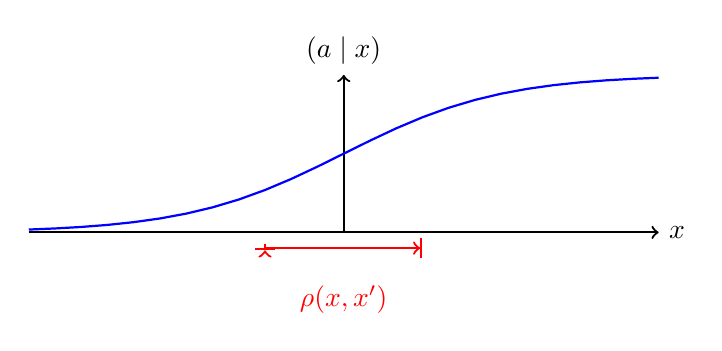
\begin{tikzpicture}[scale=2,thick,domain=-2:2]
    \draw[->] (-2,0) -- (2,0) node[right] {$x$};
    \draw[->] (0,0) -- (0,1) node[above] {$\pol(a \mid x)$};
    \draw[color=blue] plot (\x,{0.5 + 0.5 * tanh(\x)}); % node[right] {$f(x) = \frac{1}{20} \mathrm e^x$};
    \draw [|<->|,color=red] plot (-0.5,-0.1) -- node[below=1em] {$\rho(x,x')$} ++(1, 0);
  \end{tikzpicture}
\end{frame}

\begin{frame}
  \frametitle{Summary of fairness conditions}
  \begin{itemize}
  \item<1-> Calibration: Given decision, outcome doesn't depend on race.
  \item<2-> Balance: Given outcome,  decision doesn't depend on race.
  \item<3-> Similarity: Similar people should be treated similarly.
  \item<4-> Meritocracy: Better people should be treated better.
  \end{itemize}

  \begin{alertblock}{Open issues}
    \begin{itemize}
    \item<5-> Can these conditions be satisfied when $\param$ is unknown?
    \item<6-> What is ``similar'' anyway?
    \end{itemize}
  \end{alertblock}
  \uncover<7>{Our solutions: Subjective fairness and informational similarity.}
\end{frame}

\begin{frame}
  \frametitle{The Bayesian fairness framework}
  \begin{center}
    \includegraphics[width=0.5\textwidth]{../figures/bias}

    From prior and data $\Rightarrow$ belief
    $\bel(\param)$
  \end{center}
  
   \begin{definition}[Bayes rule]
     The optimal decision rule simply maximises expected utility:
     \begin{align}
       \pol^*(a \mid x) &= \argmax_a \E_\bel(U \mid a, x)
       \\
       \E_\bel(U \mid a, x) &= \int_\Param \E_\param(U \mid a, x) \dd \bel(\param)
     \end{align}
   \end{definition}
\end{frame}
\begin{frame}
  \frametitle{Example: Balanced decision rules.}
  \begin{definition}[Balanced decision rule]
    A decision rule $\pol$ is balanced with respect to $\param$ if
  \begin{align*}
    C_\param^\pol(y,z) &\defn \Pr_\param^\pol(a, z \mid y) -  \Pr_\param^\pol(a  \mid y)  \Pr_\param^\pol(z  \mid y) = 0 &&\forall x, y, z
  \end{align*}
  i.e. $a \indep z \mid y, \pol, \param$.
\end{definition}

\begin{block}{When $\param$ is unknown}

      \[
        \max_\pol \int_\Param \dd \bel(\param) [U(\param, \pol) - \lambda \max_{y, z} C_\param^\pol(y,z)]
      \]
    \end{block}
    where $\Delta$ measures dependence.
\end{frame}

\begin{frame}
\frametitle{Informational fairness}

  ``Similar people should be treated similarly''

  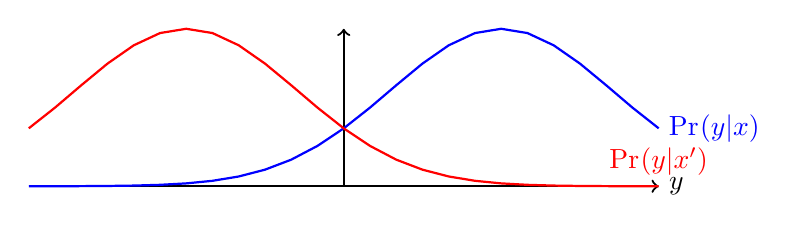
\begin{tikzpicture}[scale=2,thick,domain=-2:2]
    \draw<1->[->] (-2,0) -- (2,0) node[right] {$y$};
    \draw<1->[->] (0,0) -- (0,1);
    \draw<2->[color=blue] plot (\x,{exp(-(\x - 1)^2)}) node[right] {$\Pr_{\bel}(y|x)$};
    \draw<3->[color=red] plot (\x,{exp(-(\x + 1)^2)}) node[above] {$\Pr_{\bel}(y|x')$};
  \end{tikzpicture}
  \uncover<4->{
    \begin{block}{Thompson sampling}
      \begin{itemize}
      \item $\hat{\param} \sim \bel$
      \item $a = \argmax_a \E_{\hat{\param}} [U \mid x, a]$
      \end{itemize}
    \end{block}
    \begin{block}{Stochastic dominance sampling}
      \begin{itemize}
      \item $\hat{\param} \sim \bel$
      \item $\hat{y} \sim \Pr_\param$
      \item $\pol(a | x) = \argmax_a U(\hat{y},a)$
      \end{itemize}
    \end{block}
    
  }
\end{frame}

\begin{frame}
  \frametitle{Current status}
  \begin{itemize}
  \item Link between smoothness and independence under uncertainty.
  \item Optimality of Thompson sampling with respect to subjective meritocracy.
  \item Introduced calibrated fairness for which stochastic dominance is optimal.
  \item Application to bandit problems.
  \item More general decision settings are an open problem.
  \end{itemize}

\end{frame}







%%% Local Variables:
%%% mode: latex
%%% TeX-engine: xetex
%%% TeX-master: "notes"
%%% End:
